\vspace{1ex}
\begin{center}
  {\large\textbf{Содержание работы}}
\end{center}

\textbf{Во введении} обоснована актуальность выполненных исследований,
сформулирована цель и научная новизна диссертационной работы. Кратко изложена
структура диссертации.

\vspace{1ex}
\textbf{В первой главе} обсуждены идеи, впервые высказанные в работах
Померанчука и Чу, указавшие на возможность использования зарядово-обменных
процессов на дейтроне для определения вклада спин-зависящей части амплитуды
$np$-упругого рассеяния.

\begin{figure}[h]
  \centering
  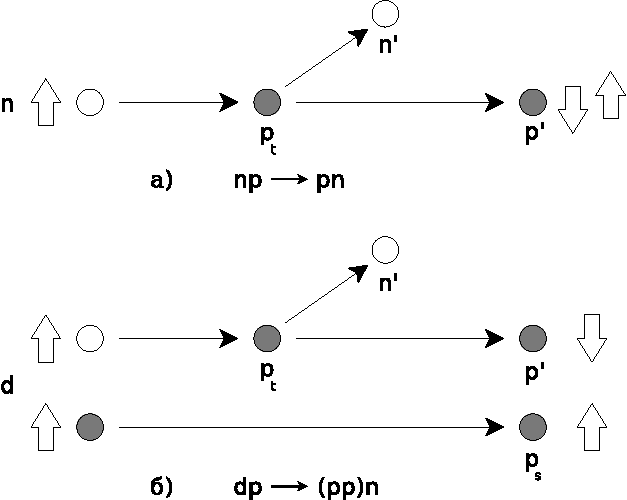
\includegraphics[width=0.60\textwidth]{np_dp_scheme-abs.pdf}
  \caption{Схематическое изображение а) элементарной реакции перезарядки
    нейтрона на протоне и б) перезарядки дейтрона на протоне-мишени.}
  \label{fig:np_dp_scheme}
\end{figure}

На рис.~\ref{fig:np_dp_scheme} схематически изображены два процесса:
элементарная реакция перезарядки нейтрона на протоне \np и реакция перезарядки
дейтрона на протоне-мишени \dpchex. Здесь в скобках два протона, связанные с
падающим дейтроном, а именно, протон-спектатор и протон от квази-$np$
перезарядки, т.е. перезарядки нейтрона (связанного в дейтроне) на
протоне-мишени. Вертикальными стрелками обозначены направления спинов нуклонов
относительно произвольной оси квантования.

В случае реакции перезарядки нейтрона на протоне (рис.~\ref{fig:np_dp_scheme}а)
возможны оба направления спина рассеянного протона. В процессе перезарядки
дейтрона на протоне (рис.~\ref{fig:np_dp_scheme}б) образуется симметричная
по заряду система из двух протонов с малым относительным импульсом. В силу
принципа Паули (статистика Ферми"--~Дирака для полуцелых спинов) при сохранении
пространственной симметрии, антисимметричность полной волновой функции двух
протонов будет достигаться только в случае переворота спина рассеянного протона.
Дейтрон в данном случае выступает как <<спиновый фильтр>>, а спин-зависящая
часть амплитуды элементарной $np$-перезарядки проявляется через вероятность
реакции перезарядки на дейтроне.

Математический формализм, используемый для определения вклада спин-зависящей
части амплитуды $np$-рассеяния из процесса перезарядки на дейтроне, был развит
в работах Дина и др. Дифференциальное поперечное сечение \np рассеяния может
быть представлено в виде суммы спин-независящей (индекс {\small$SI$}) и
спин-зависящей (индекс {\small$SD$}) частей
\begin{equation}
  \label{eq:np}
  (d\sigma/dt)_{\np} = (d\sigma/dt)^{SI}_{\np} + (d\sigma/dt)^{SD}_{\np}\,,
\end{equation}
где $t$~--- квадрат четырёхмерного переданного импульса.

В рамках импульсного приближения соотношение между дифференциальными сечениями
перезарядки дейтрона на протоне \dpchex и элементарной перезарядки \np можно
записать как
\begin{equation}
  \label{eq:dpnp}
  (d\sigma/dt)_{\dpchex} = [1-F_d(t)]\,(d\sigma/dt)^{SI}_{\np} +
  [1-1/3\,F_d(t)]\,(d\sigma/dt)^{SD}_{\np}\,,
\end{equation}
где $F_d(t)$ обозначает формфактор дейтрона. При нулевом переданном импульсе
($t=0$), когда $F_d(0) = 1$, дифференциальное поперечное сечение перезарядки на
дейтроне будет равно
\begin{equation}
  \label{eq:dpnp0}
  (d\sigma/dt)_{\dpchex} = 2/3\,(d\sigma/dt)^{SD}_{\np}\,.
\end{equation}

Таким образом, имеется возможность определения части взаимодействия нейтрона и
протона, которая полностью зависит от спина. Реакция перезарядки
неполяризованного дейтрона на неполяризованном протоне-мишени при нулевой
передаче импульса определяется спин-зависящей частью перезарядки нейтрона на
протоне. Анализ процесса \dpchex при малых переданных импульсах, близких к нулю,
позволяет оценить вклад спин-зависящей части амплитуды реакции перезарядки \np.

В конце главы обсуждены избранные исследования с дейтронами. Рассмотрение
экспериментальных данных по определению спин-зависящей части амплитуды \np
перезарядки показало, что в настоящее время существует более или менее полная
картина в интервале энергий до сотен~МэВ. В области энергий 1~ГэВ и выше
экспериментальная информация скудна и продолжение исследований в этой области
энергий остаётся весьма актуальным.

\vspace{1ex}
\textbf{Вторая глава} посвящена изучению зарядово-обменных процессов в
дейтрон-протонных взаимодействиях. Экспериментальный материал был получен с
помощью 100-см водородной пузырьковой камеры на синхрофазотроне ЛВЭ ОИЯИ.
Камера была облучена выведенным из ускорителя пучком дейтронов с импульсом
3.35~ГэВ/с. После стандартной процедуры просмотра, измерений и идентификации
каналов в условиях 4$\pi$-геометрии была получена лента суммарных результатов
(DST), которая содержит почти четверть миллиона событий.

Приблизительно половину всех событий дейтрон-протонных столкновений составляла
реакция безмезонного развала дейтрона \dpfrag. Эта реакция может идти как
\dpchex~--- реакция перезарядки с изменением зарядового состояния
протона-мишени, или \dpret~--- реакция прямого развала дейтрона с сохранением
заряда. Разделение этих двух классов событий можно видеть на
рис.~\ref{fig:chex_ret_t}, где приводятся их распределения по величине квадрата
переданного четырёхмерного импульса $t$. К перезарядке отнесены события, в
которых самым быстрым из вторичных нуклонов в системе покоя дейтрона являлся
нейтрон. Число таких событий равно 17512, что соответствует поперечному сечению
(5.85~$\pm$~0.05)~мб. При этом миллибарн-эквивалент события определялся исходя
из полного сечения $dp$-взаимодействий с учётом потерь событий упругого
рассеяния \dpela. Систематическая ошибка, связанная с оценкой потерь событий в
упругом $dp$-рассеянии, составляла около 4~$\%$.

\begin{figure}[h]
  \centering
  \vspace{-2ex}
  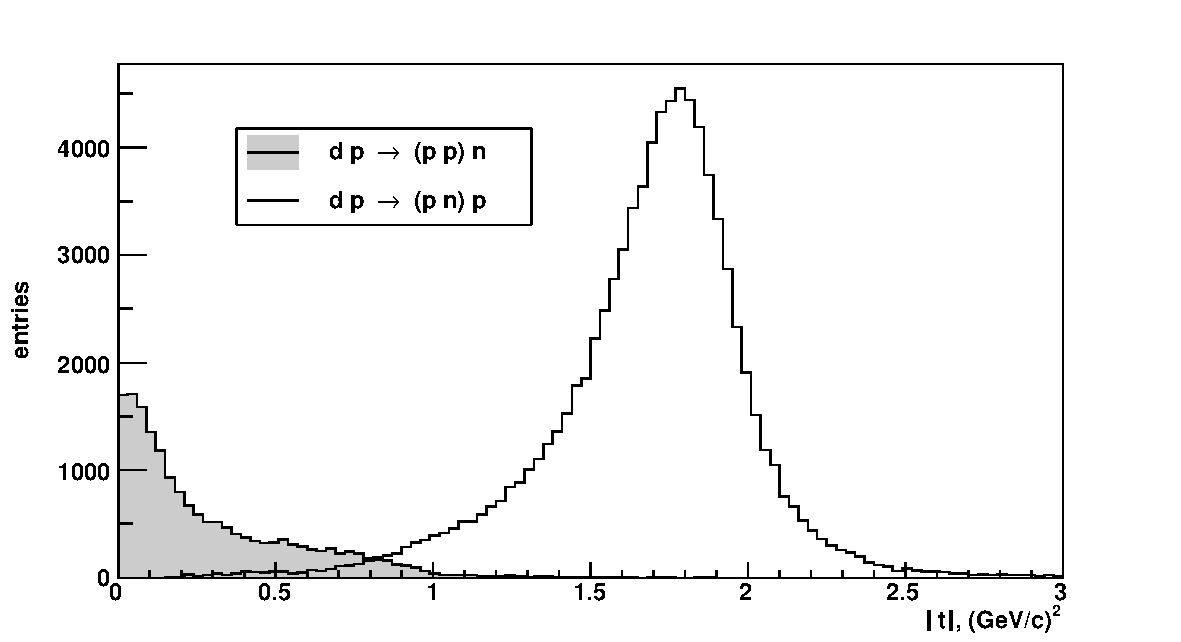
\includegraphics[width=0.97\textwidth]{chex_ret_t-abs.pdf}
  \vspace{-2ex}
  \caption{Распределения событий реакции \dpfrag по квадрату четырёхмерного
    переданного импульса $|t|$ от протона-мишени к нейтрону.}
  \label{fig:chex_ret_t}
\end{figure}

Формулы~\eqref{eq:dpnp} и~\eqref{eq:dpnp0} выведены в определённых
предположениях. Чтобы воспользоваться этими выражениями, мы должны выполнить по
крайней мере два условия, а именно, работать в области малых переданных
импульсов квази-упругого $np$-рассеяния и принять справедливость импульсного
приближения. В работе показано, что при релятивистских энергиях эти
предположения оправданы.

Условие импульсного приближения предполагает подавление взаимодействия в
конечном состоянии (ВКС). При экспериментальном исследовании механизма ВКС
наблюдалось, что этот эффект сильно проявляется в асимметрии распределений по
углу $\alpha = \arccos{\bigl((\vec{p_s}\,\vec{q})/
  (|\,\vec{p_s}\,|\,|\,\vec{q}\,|)\bigr)}$, где $\vec{p_s}$~--- импульс
спектатора, а $\vec{q}$~--- трёхмерная передача импульса от налетающего нуклона
к рассеянному. В области малых переданных импульсов $|t| < 0.1$ (ГэВ/с)$^2$ и
импульсов спектаторов, меньших приблизительно 0.1~ГэВ/с, асимметрии по углу
$\alpha$, вызванные ВКС, практически отсутствуют (близки к нулю). Это хорошо
видно из рис.~\ref{fig:asymmetry_alpha}, как для прямого развала дейтрона
(сплошные кружки), так и для развала дейтрона с перезарядкой (пустые кружки),
где асимметрия менее выразительна и становится ненулевой при заметно больших
значениях импульса спектатора. Такое поведение асимметрии по углу $\alpha$
указывает на возможность применения импульсного приближения в интересующей нас
области малых переданных импульсов и малых импульсов спектаторов.

\begin{figure}[h]
  \centering
  \vspace{-2ex}
  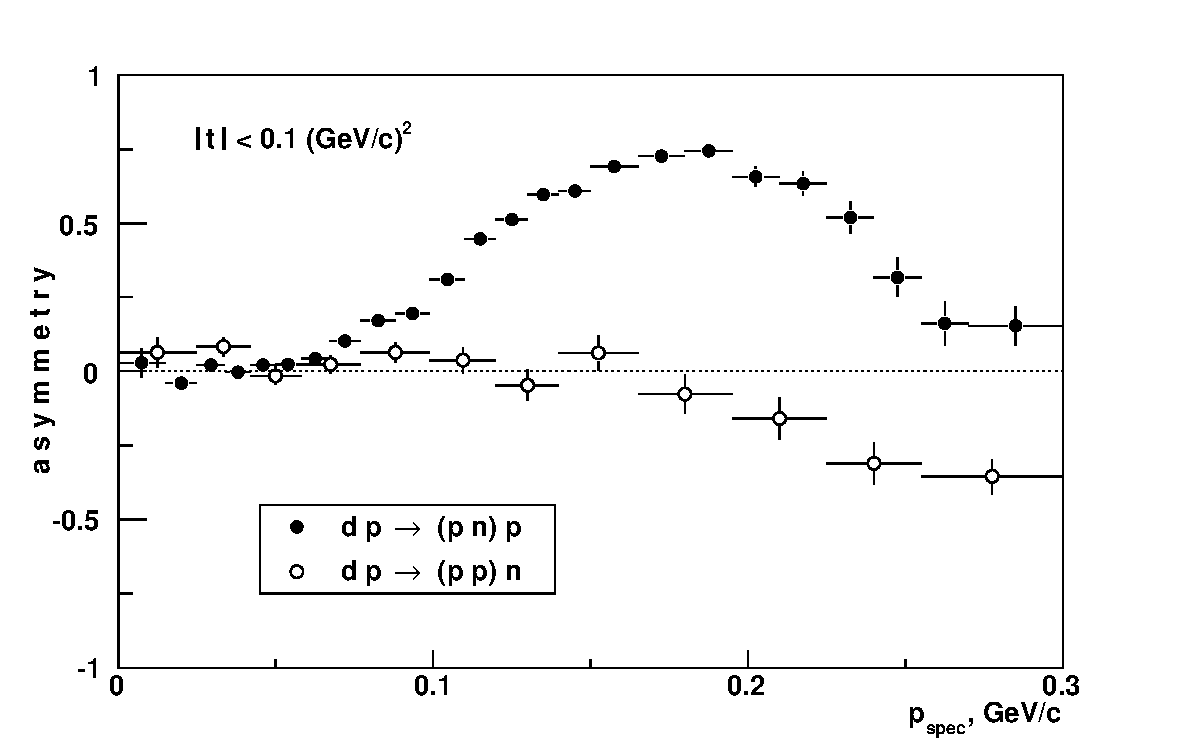
\includegraphics[width=0.91\textwidth]{asymmetry_alpha-abs.pdf}
  \vspace{-2ex}
  \caption{Зависимость асимметрии по углу $\alpha$ от импульса спектатора
    $p_{spec}$ в системе покоя дейтрона.}
  \label{fig:asymmetry_alpha}
\end{figure}

Вышеуказанным условиям можно одновременно удовлетворить, отбирая такие события,
для которых в лабораторной системе координат (быстрый дейтрон падает на
покоящуюся протонную мишень) два быстрых протона из реакции перезарядки \dpchex
вылетают под малыми углами по отношению к падающему дейтрону и с импульсами
близкими к половине импульса дейтрона. При этом они могут быть надёжно
зарегистрированы и хорошо измерены. Заметим, что поставленная задача может быть
экспериментально выполнена только при наличии ускоренных дейтронов. В случае
падающего быстрого протона на покоящуюся дейтронную мишень, вторичные протоны из
такой реакции перезарядки $pd \rightarrow n(pp)$ будут слишком медленными, чтобы
их зарегистрировать, а сама реакция не может быть идентифицирована. Преимущество
изучения дейтрон-протонных взаимодействий (так называемая обратная геометрия)
является очевидным в отличие от протон-дейтронных взаимодействий.

\begin{figure}[h]
  \centering
  \vspace{-2ex}
  % 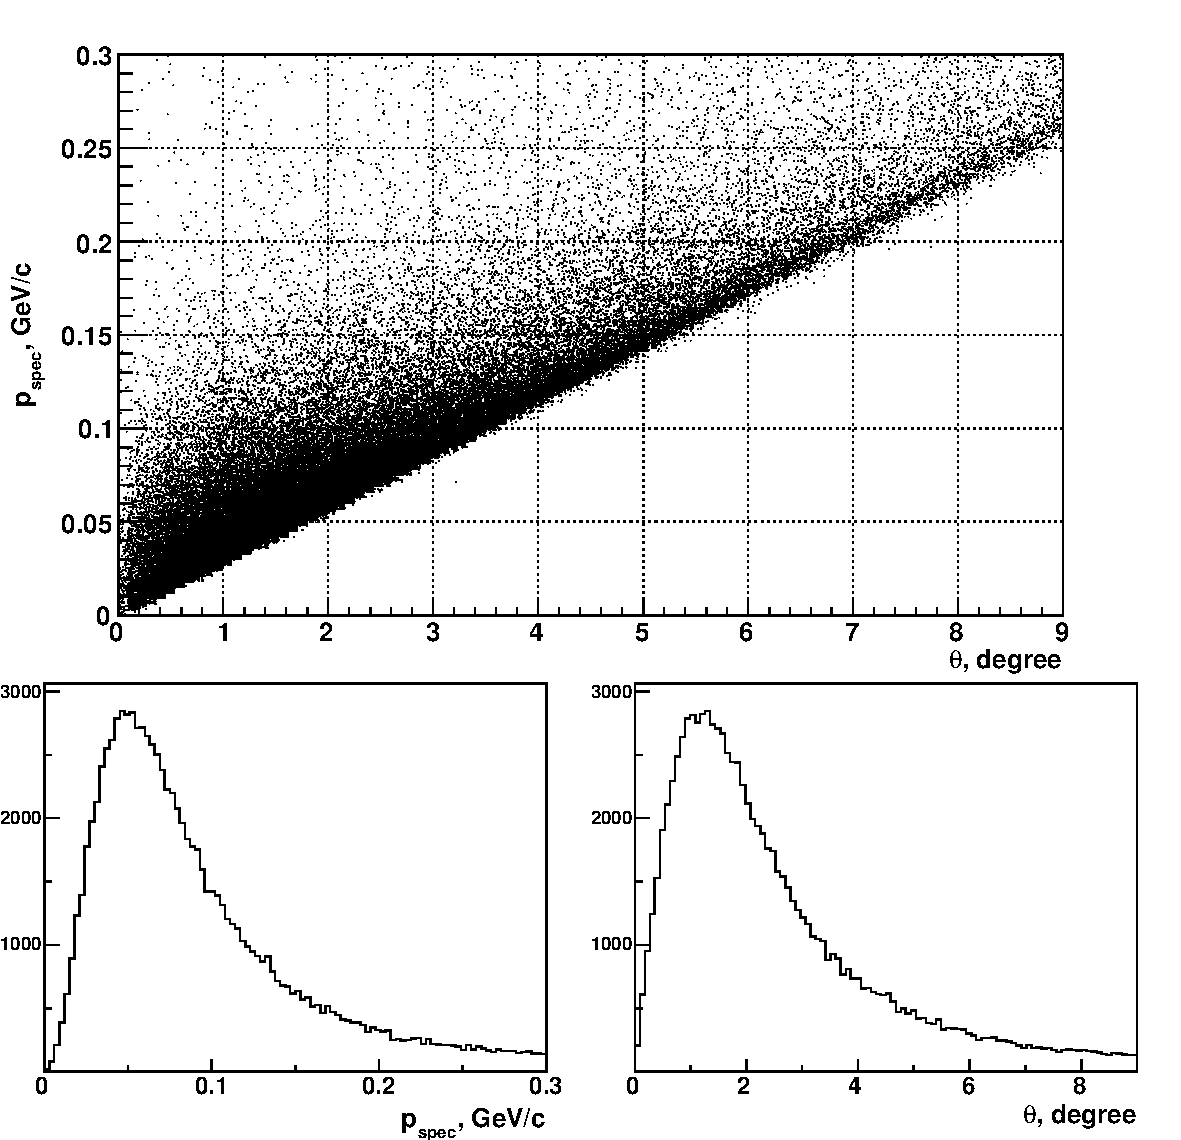
\includegraphics[width=0.82\textwidth]{theta_p-abs.pdf}
  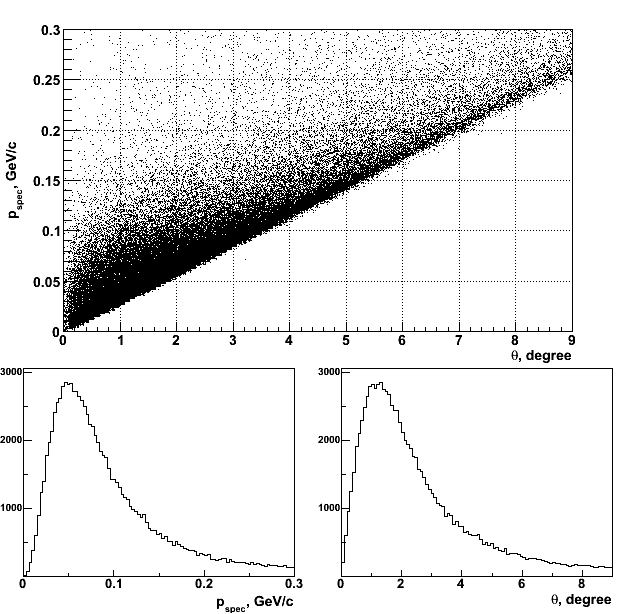
\includegraphics[width=0.82\textwidth]{theta_p-abs.png}
  \vspace{-2ex}
  \caption{Зависимость полярного угла вылета $\theta$ нуклона-спектатора от его
    импульса $p_{spec}$ из реакции развала дейтрона на протоне. Нижние
    распределения~--- проекции на соответствующие оси.}
  \label{fig:theta_p}
\end{figure}

На рис.~\ref{fig:theta_p} показана кинематическая зависимость (и её проекции)
между полярным углом вылета нуклона-спектатора в лабораторной системе координат
и его импульсом в системе покоя дейтрона. Видно, что при углах меньших
$\sim$~5$^{\,\circ}$, или при импульсе спектатора меньше $\sim$~0.15~ГэВ/с,
лежит основная часть событий, соответствующих квази-нуклонному рассеянию. В
случае, когда передача четырёхмерного импульса стремится к нулю
$|t| \rightarrow 0$, два быстрых протона из реакции перезарядки в лабораторной
системе координат имеют практически одинаковые импульсы близкие к половине
импульса дейтрона $p_{p_1} \simeq p_{p_2} \simeq (1/2)\,p_d$.

Для набора пар протонов, попадающих в конус с раствором меньше~5$^{\,\circ}$,
строилось распределение сечения $d\sigma/dt$ с учётом миллибарн-эквивалента
события и поправки, равной отношению полного числа спектаторных нуклонов к числу
спектаторов в выбранном конусе. Дифференциальное поперечное сечение
$(d\sigma/dt)_{\dpchex}$ изучаемой реакции перезарядки на дейтроне при малых
значениях $|t|$ и импульсе дейтрона 3.35~ГэВ/с приведено на
рис.~\ref{fig:dp_two_protons}. Распределение аппроксимировалось и
экстраполировалось к $t=0$, что дало значение
$(d\sigma/dt)_{\dpchex}\,|\,_{t=0} = 30.2 \pm 4.1$~мб/(ГэВ/с)$^{2}$.

\begin{figure}[h]
  \centering
  \vspace{-2ex}
  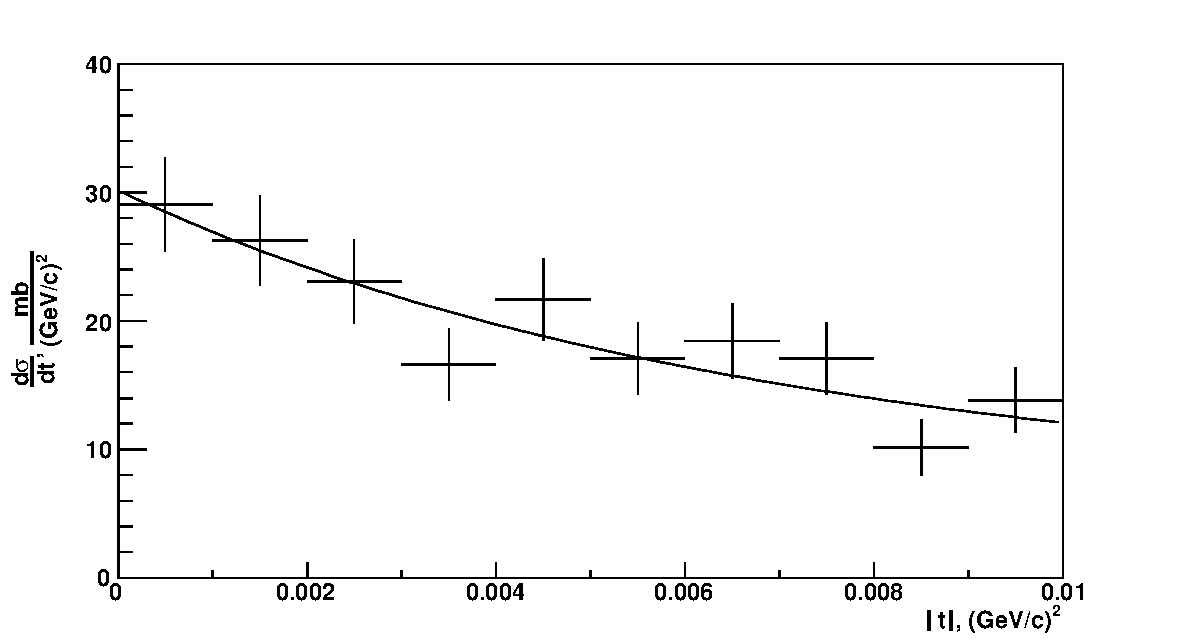
\includegraphics[width=0.97\textwidth]{dp_two_protons-abs.pdf}
  \vspace{-2ex}
  \caption{Распределение дифференциального поперечного сечения реакции с обменом
    заряда \dpchex при малых значениях $|t|$.}
  \label{fig:dp_two_protons}
\end{figure}

Проведённый анализ экспериментальных данных по реакции перезарядки дейтрона на
протоне-мишени, даёт возможность получить информацию о спиновой зависимости
обменного $np$-рассеяния. Для ответа, на интересующий нас вопрос о вкладе
спин-зависящей части амплитуды элементарного \np процесса, необходимо кроме
измеренного дифференциального поперечного сечения
$(d\sigma/dt)_{\dpchex}\,|\,_{t=0}$, привлечь и результаты экспериментов по
измерению дифференциального сечения $(d\sigma/dt)_{\np}$ реакции элементарной
перезарядки \np при $|t|=0$. В работе было показано, что среди имеющихся в
литературе экспериментальных данных для $np$-рассеяния, измерения сделанные
Бизардом~и~др. на ускорителе Сатурн являются наиболее корректными и самыми
близкими по энергии. На их основе, для импульса 1.675~ГэВ/с на нуклон, была
получена величина
$(d\sigma/dt)_{\np}\,|\,_{t=0} = 54.7 \pm 0.2$~мб/(ГэВ/с)$^{2}$.

Введём отношение $R_{\np}$ дифференциальных сечений для реакции перезарядки на
дейтроне \dpchex и элементарной перезарядки \np
\begin{equation}
  R_{\np} = \frac{(d\sigma/dt)_{\dpchex}}{(d\sigma/dt)_{\np}}\,.
\end{equation}
При нулевом переданном импульсе $|t|=0$ отношение $R_{\np}$, исходя из
формулы~\eqref{eq:dpnp0}, определяет вклад спин-зависящей части амплитуды
перезарядки нейтрона на протоне и его можно записать как
\begin{equation}
  R_{\np} = \frac{2}{3}\,\frac{(d\sigma/dt)^{SD}_{\np}}{(d\sigma/dt)_{\np}}\,.
\end{equation}
Если бы дифференциальное поперечное сечение перезарядки на дейтроне при $|t|=0$
равнялось $2/3$ от дифференциального сечения элементарной \np перезарядки при
$|t|=0$, то это бы означало, согласно выше приведённым формулам, что амплитуда
элементарной перезарядки являлась бы полностью спин-зависящей. Однако на
эксперименте такой закономерности не наблюдается.

Из измеренного нами
$(d\sigma/dt)_{\dpchex}\,|\,_{t=0} = 30.2 \pm 4.1$~мб/(ГэВ/с)$^{2}$ и
$(d\sigma/dt)_{\np}\,|\,_{t=0} = 54.7 \pm 0.2$~мб/(ГэВ/с)$^{2}$, определённого
на основе данных Бизардa~и~др., получаем значение отношения дифференциальных
поперечных сечений
\begin{equation}
  R_{\np} = 0.55 \pm 0.08\,,
\end{equation}
свидетельствующее о преобладающем вкладе спин-зависящей части амплитуды \np
рассеяния. На рис.~\ref{fig:R_np} показана зависимость величины $R_{\np}$ от
кинетической энергии нейтрона в сравнении с результатами других экспериментов.
Видно, что полученное нами значение находится в согласии, как с более ранними,
так и с недавно опубликованными результатами группы Дельта-Сигма при более
высоких энергиях.

\begin{figure}[h]
  \centering
  \vspace{-1ex}
  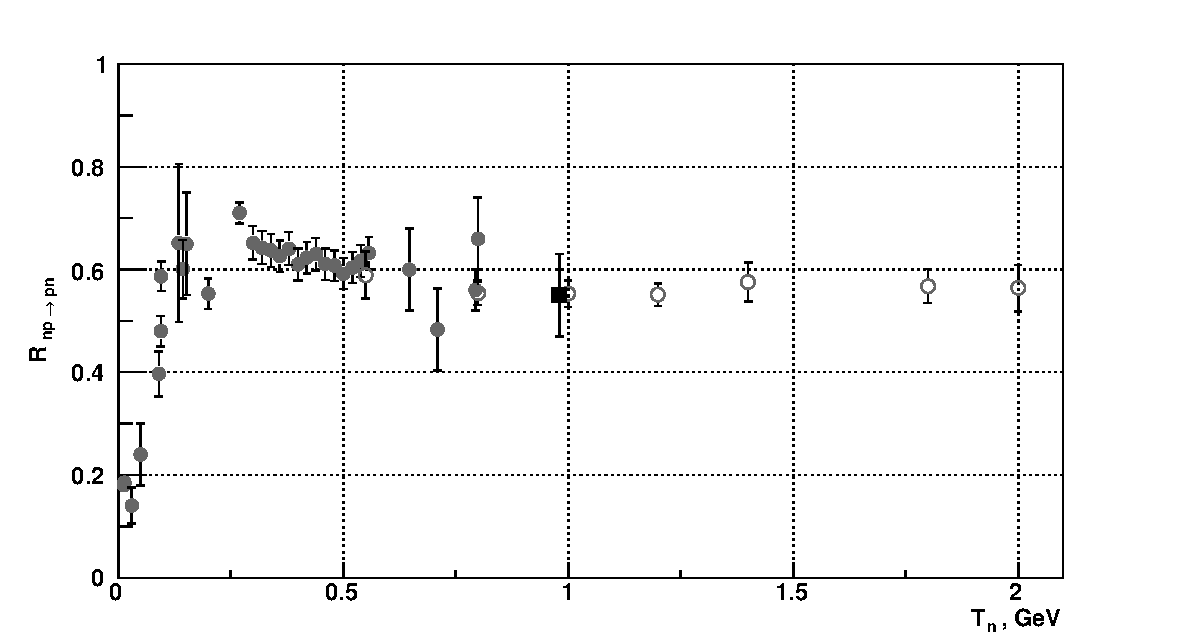
\includegraphics[width=0.99\textwidth]{R_np-abs.pdf}
  \vspace{-2ex}
  \caption{Зависимость величины $R_{\np}$ от кинетической энергии нейтрона
    $T_n$. Сплошные кружки представляют значения, полученные в более ранних
    экспериментах, квадратик ($T_n = 0.98$~ГэВ)~--- определённое нами значение,
    пустые кружки~--- недавно опубликованные результаты эксперимента
    Дельта-Сигма.}
  \label{fig:R_np}
\end{figure}

Это первая и единственная работа выполненная на пучке дейтронов. Следует
отметить, что все более ранние работы на эту тему были выполнены на пучках
нейтронов довольно широкого импульсного спектра, полученных коллимированием
вторичных нейтронов. Позже, в эксперименте Дельта-Сигма, где использовались
квази-монохроматические нейтроны от стриппинга выведенных из ускорителя
монохроматических дейтронов, удалось существенно сузить спектр такого
нейтронного пучка.

\vspace{1ex}
\textbf{В третьей главе} подробно описывается экспериментальная установка
СТРЕЛА, предназначенная для исследования зарядово-обменных процессов в
дейтрон-протонных столкновениях в области энергий выше 1~ГэВ. Анализ
$dp$-взаимодействий, полученных с помощью камерной методики, позволил предложить
схему электронного эксперимента. Появилась возможность изучения интересующего
нас процесса на большой статистике событий при использовании выведенного пучка
ускоренных дейтронов на Нуклотроне ЛФВЭ ОИЯИ.

Была предложена довольно простая (изучение процесса с малой множественностью
вторичных частиц и предсказуемой кинематикой) схема эксперимента,
а именно~--- одноплечевой спектрометр с достаточно узкой апертурой
(рис.~\ref{fig:strela_scheme}). Пучок дейтронов падает на мишень, анализирующий
магнит разводит в пространстве вторичные заряженные частицы (протоны) и
непровзаимодействовавшие дейтроны. Предлагаемая схема электронного эксперимента
позволяет регистрировать пары протонов с малым углом раствора, имеющие импульс
равный приблизительно половине импульса дейтрона. Этим обеспечивается отбор
событий под нулевым углом по отношению к первичному пучку, что соответствует
малому переданному импульсу ($t \simeq 0$). Таким образом, реализуются
необходимые условия для выделения изучаемого процесса.

\begin{figure}[h]
  \centering
  \vspace{2ex}
  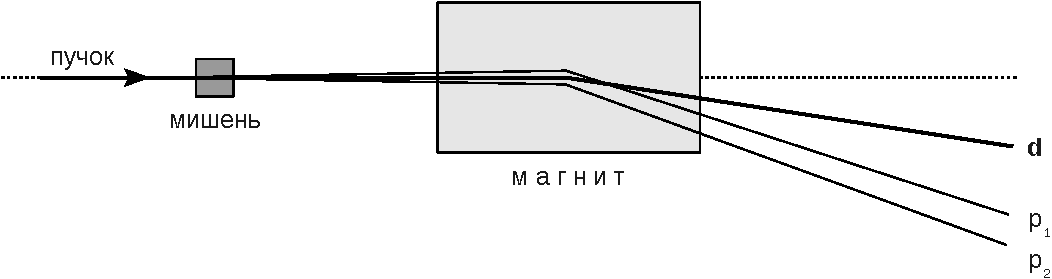
\includegraphics[width=1.00\textwidth]{strela_scheme-abs.pdf}
  \caption{Схема эксперимента с использованием одноплечевого спектрометра,
    обеспечивающая отбор событий с вылетом из мишени двух протонов с близкими
    импульсами в переднем направлении.}
  \label{fig:strela_scheme}
\end{figure}

Выбор конкретной геометрии эксперимента был выполнен на основе расчётов методом
Монте"--~Карло генерации с помощью программного пакета GEANT. Опираясь на данные
по $dp$-взаимодействиям, полученные на водородной пузырьковой камере, был
промоделирован вариант эксперимента для спектрометра, используя в качестве
входных данных реальные события.

В результате была создана экспериментальная установка СТРЕЛА. Основными
элементами установки являются блоки дрейфовых камер в качестве координатных
детекторов, электроника считывания информации, сцинтилляционные счётчики,
используемые для запуска установки и анализирующий магнит. На
рис.~\ref{fig:strela_setup} приведена схема расположения всех элементов
установки.

\begin{figure}[h]
  \centering
  \vspace{-6ex}
  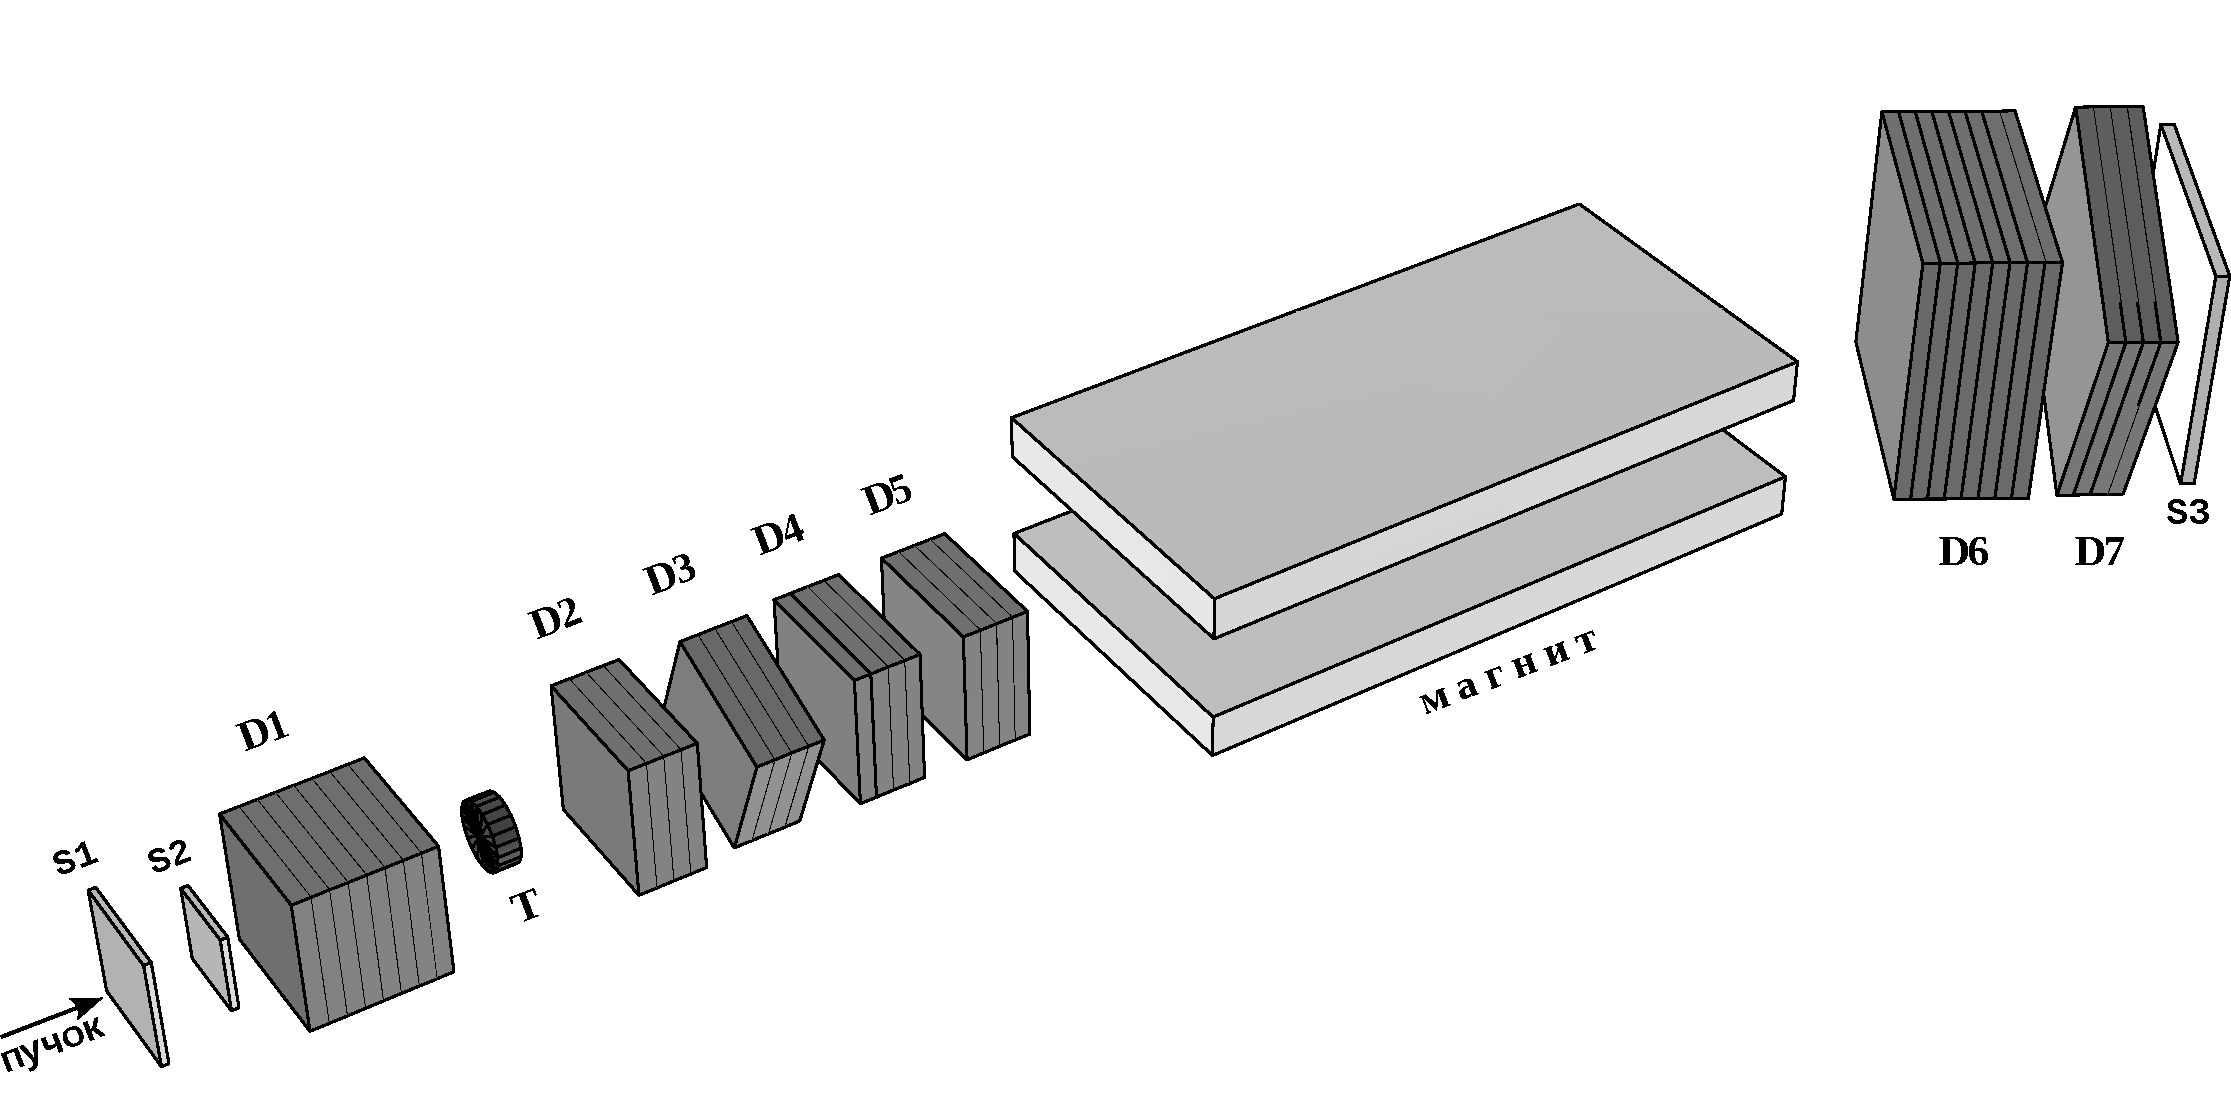
\includegraphics[width=1.00\textwidth]{strela_setup.pdf}
  \vspace{-2ex}
  \caption{Экспериментальная установка СТРЕЛА. D1--D5~--- блоки <<маленьких>>
    дрейфовых камер с размером рабочей области 12.5~$\times$~12.5~см$^2$,
    D6--D7~--- блоки <<больших>> камер с размером 25.0~$\times$~25.0~см$^2$,
    S1--S3~--- сцинтилляционные счётчики,  Т~--- мишень.}
  \label{fig:strela_setup}
\end{figure}

В настоящее время используется 36 плоскостей дрейфовых камер, объединённых в 7
блоков. Каждый блок состоит из четырёх или восьми плоскостей дрейфовых камер с
различной ориентацией проволочек. Длина дрейфового промежутка во всех камерах
равна 21~мм. Камеры в блоке располагаются таким образом, что сигнальные
проволочки в соседних плоскостях сдвинуты относительно друг друга на 21~мм в
направлении перпендикулярном оси пучка. Такое расположение проволочек позволяет
устранить лево-правую неоднозначность в определении пространственных координат
треков частиц. В данной главе подробно освещены принципы работы и конструкции
используемых дрейфовых камер, как наиболее важных элементов установки.

Число всех регистрируемых сигналов с проволочек составляет 162. На каждой камере
установлены платы с микросхемами, в которых осуществляется усиление,
формирование и дискриминация входных сигналов от сигнальных проволочек дрейфовых
камер. Сформированные сигналы поступают на входы TDC модулей для оцифровки.
Полученная информация передаётся по оптической линии в персональный компьютер
для дальнейшей обработки.

На установке СТРЕЛА, для организации системы сбора экспериментальных данных
применяется несколько модулей быстрой электроники в формате стандарта VME.
Данный стандарт предполагает создание высокопроизводительных вычислительных
систем модульного типа на основе унифицированной магистрали и обладает
достаточной универсальностью и расширяемостью. Упрощённая блок-схема системы
сбора данных установки показана на рис.~\ref{fig:modules_VME.pdf}.

\begin{figure}[h]
  \centering
  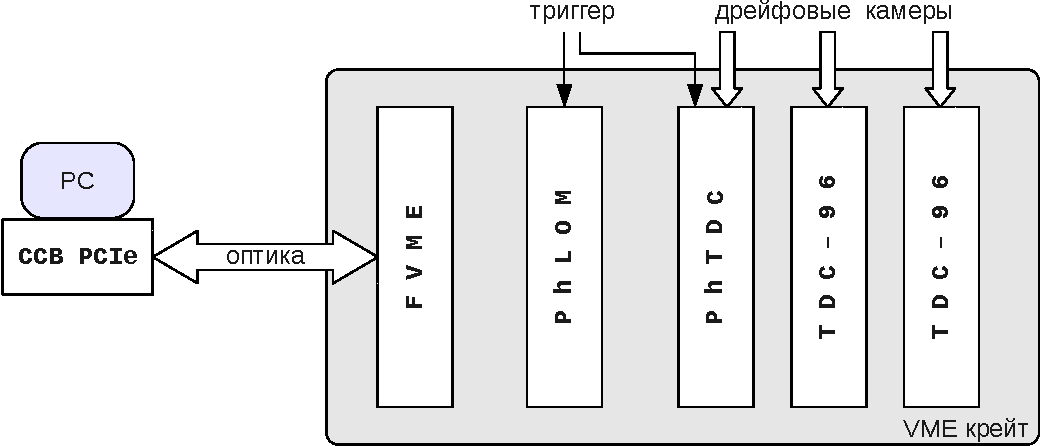
\includegraphics[width=0.81\textwidth]{modules_VME-abs.pdf}
  \caption{Блок-схема системы сбора данных на установке. Сформированные сигналы
    с дрейфовых камер оцифровываются в модулях время-цифрового преобразования
    TDC-96 и PhTDC. Триггерный сигнал поступает на модули PhLOM и PhTDC.
    Интерфейсный FVME контроллер обеспечивает связь VME с удалённым компьютером
    по высокоскоростной оптической линии.}
  \label{fig:modules_VME.pdf}
\end{figure}

Система запуска (триггер) установки должна обеспечить набор событий реакции
развала дейтрона. В нашем случае регистрируются однопротонные события из
реакции прямого развала дейтрона \dpret и два протона с близкими импульсами и
малым углом раствора из реакции перезарядки дейтрона на протоне \dpchex (развал
дейтрона с зарядовым обменом). Запуск установки осуществлялся с помощью трёх
триггерных сцинтилляционных счётчиков S1--S3 (рис.~\ref{fig:strela_setup}),
которые определяют аксептанс установки и вырабатывают сигнал для открытия
временного окна регистрации сигналов с дрейфовых камер и запуска системы сбора
данных.

Изучение характеристик блоков дрейфовых камер экспериментальной установки СТРЕЛА
было проведено при облучении полиэтиленовой мишени коллимированным пучком
дейтронов с импульсом 3.5~ГэВ/с на канале ВП-1 ускорительного комплекса
Нуклотрона ЛФВЭ ОИЯИ. Аппаратура установки проверялась в течение почти двух
суток. В результате облучения было набрано несколько миллионов триггеров для
последующего анализа.

\vspace{1ex}
\textbf{В четвёртой главе} представлены алгоритмы для восстановления треков в
дрейфовых камерах. Разработан и протестирован на реальных событиях полный
комплекс программ обработки и анализа экспериментальных данных. Исходный код
программ написан полностью на языке С++ с использованием библиотек ROOT, что
делает их универсальными и модульными.

Выбор дрейфовых камер в качестве координатных детекторов спектрометра на
установке СТРЕЛА обусловлен необходимостью получения высокого пространственного
разрешения. Применение дрейфовых камер требует определения соотношения между
измеренным временем дрейфа $t$ проходящей частицы и его преобразованием в
расстояние $r$ относительно данной сигнальной проволочки, так называемая
$r(t)$-зависимость. Неравномерность напряжённости электрического поля вдоль
траектории дрейфа электронов приводит к изменению величины скорости дрейфа, и
соответственно, к дифференциальной нелинейности $r(t)$-зависимости. Это возможно
в конструкции используемых дрейфовых камер, где напряжённость электрического
поля вдоль траектории дрейфа задаётся резистивной сборкой, резисторы которой
имеют разброс в несколько процентов.

Получение правильного соотношения между измеренным временем дрейфа и его
преобразованием в расстояние является одной из важнейших задач при
восстановлении треков в камерах. В ходе подготовки эксперимента была разработана
итеративная процедура определения $r(t)$-зависимости с использованием трековой
информации, называемая автокалибровкой. С каждой итерацией получается новая,
подправленная функция преобразования времени дрейфа в расстояние, с которой
вновь выполняется реконструкция трека.

Пространственное разрешение дрейфовых камер определяется шириной распределения
трекового остатка $\triangle r$ данной камеры. Трековый остаток (residual)~---
это разница между расстоянием полученным преобразованием времени дрейфа
$r(t)$-зависимостью, и расстоянием восстановленного трека от сигнальной
проволочки камеры. Ожидаемое среднее значение $\triangle r = 0$. Как меняется
распределение трекового остатка в зависимости от номера итерации автокалибровки,
показано на рис.~\ref{fig:per_iterative}. Видно, что с ростом номера итерации
$\triangle r$ стремится к нулю, а ширина распределения уменьшается.

\begin{figure}[h]
  \centering
  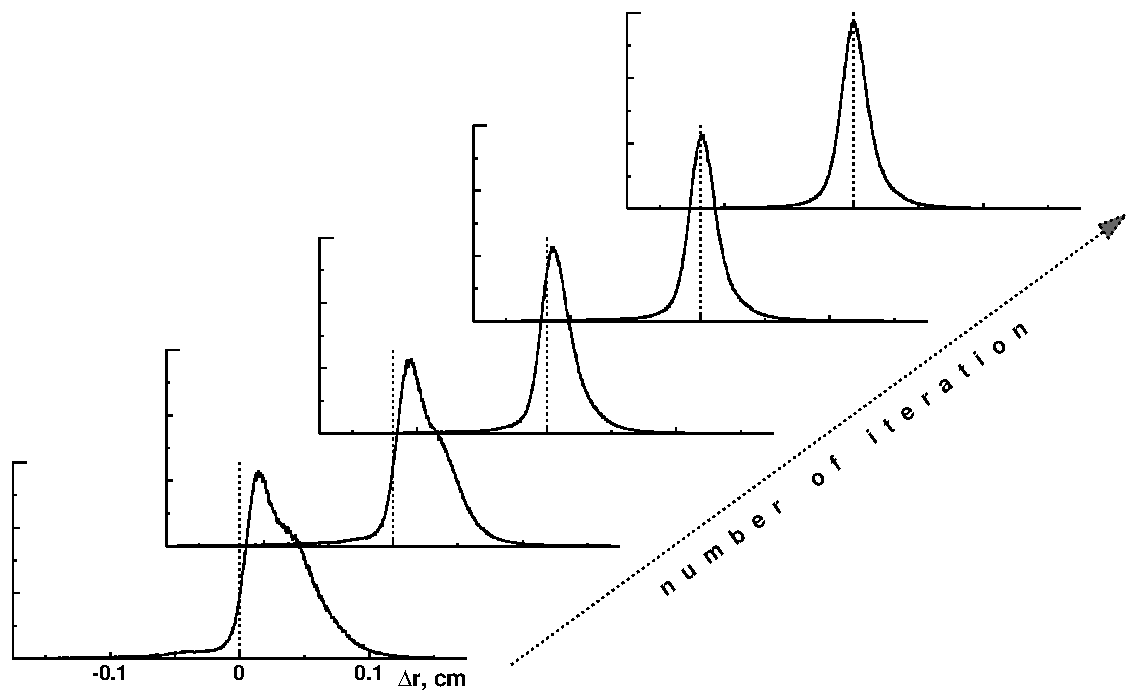
\includegraphics[width=1.00\textwidth]{c_per_iterative-abs.pdf}
  \caption{Изменение распределения трекового остатка $\triangle r$ в зависимости
    от номера итерации автокалибровки в дрейфовой камере.}
  \label{fig:per_iterative}
\end{figure}

Созданная процедура автокалибровки улучшает пространственное \linebreak
разрешение дрейфовых камер, доводя его среднее значение до 90--120~мкм.
Полученные характеристики трековых детекторов позволяют осуществить
исследования зарядово-обменных процессов в дейтрон-протонных взаимодействиях на
установке СТРЕЛА.

\vspace{1ex}
\textbf{В заключении} кратко сформулированы основные результаты и выводы
диссертации.

\vspace{1ex}
\begin{center}
  \textbf{Список публикаций по теме диссертации}
\end{center}

\renewcommand\bibsection{}
\renewcommand\baselinestretch{1.125}
\small
\bibliographystyle{gost705}
\bibliography{musinsky_references}

%%% Local Variables:
%%% mode: latex
%%% TeX-master: "musinsky_abstract"
%%% coding: utf-8
%%% End:
